\documentclass{standalone}
\usepackage{pgfplots}
\pgfplotsset{compat=1.17}
\begin{document}

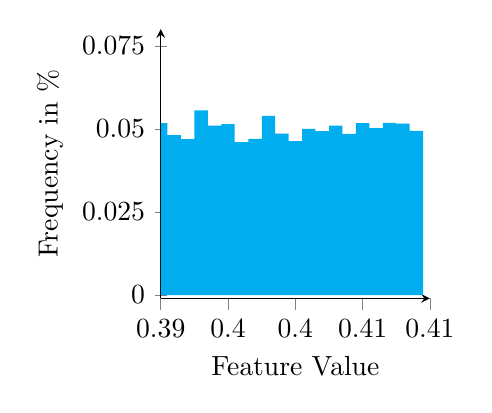
\begin{tikzpicture}

    \begin{axis}[
        width=5cm,height=5cm,
        axis lines=left,
        scaled y ticks=false,
        ylabel={Frequency in \%},
        xlabel={Feature Value},
        legend style={at={(0.5,-0.1)},
        anchor=north,legend columns=-1},
        ybar=0pt,
        bar width=4.8pt,
        ymin=-0.001,
        ymax=0.080,
        ytick={0, 0.025, 0.05, 0.075},
        yticklabels={$0$, $0.025$, $0.05$, $0.075$},
        xmin=0.39,
        xmax=0.41,
        % xtick={0.2, 0.4, 0.6,/ 0.8, 1.0}
    ]
    \addplot[draw opacity=0.0, fill=cyan]
        coordinates {
            (0.3900009, 0.051699999999999996)
            (0.3910007, 0.0481)
            (0.3920006, 0.046900000000000004)
            (0.3930004, 0.0556)
            (0.3940003, 0.051)
            (0.3950001, 0.051399999999999994)
            (0.396, 0.046)
            (0.3969998, 0.047)
            (0.3979997, 0.053899999999999997)
            (0.3989995, 0.048600000000000004)
            (0.3999994, 0.0463)
            (0.4009993, 0.05)
            (0.4019991, 0.0493)
            (0.402999, 0.051)
            (0.4039988, 0.048499999999999995)
            (0.4049987, 0.051699999999999996)
            (0.4059985, 0.050199999999999995)
            (0.4069984, 0.0518)
            (0.4079982, 0.0516)
            (0.4089981, 0.049400000000000006)
            };

    % \legend{$xX$}
    \end{axis}

\end{tikzpicture}

\end{document}